\documentclass[a4paper, 14pt,russian]{extarticle}

\usepackage[russian]{babel}
\usepackage[T2A]{fontenc}
\usepackage[utf8]{inputenc}
%Соответствующий математический шрифт для Times new roman
\usepackage{newtxmath}
\usepackage{fontspec} 
\usepackage{multirow}
%\usepackage{polyglossia}
%Times new roman
\defaultfontfeatures{Ligatures={TeX},Renderer=Basic} 
\setmainfont[Ligatures={TeX,Historic}]{Times New Roman}
\setmainfont{Times New Roman}
\setsansfont{Arial}
\setmonofont{Courier New}
\newfontfamily\cyrillicfont[Script=Cyrillic]{Times New Roman}
\newfontfamily\cyrillicfontsf[Script=Cyrillic]{Arial}
\newfontfamily\cyrillicfonttt[Script=Cyrillic]{Courier New}

%\setdefaultlanguage{russian}

%Геометрия
\usepackage{geometry}
\geometry{top=20mm}
\geometry{bottom=15mm}
\geometry{left=20mm}
\geometry{right=15mm}
\usepackage{setspace}
%Нормальные дроби через запятую
\usepackage{ncccomma}

\newcommand{\changefont}{%
	\fontsize{12}{11}\selectfont
}

%Заголовки
\usepackage{fancyhdr}
\pagestyle{fancy}
\fancyhf{}
%\renewcommand{\sectionmark}[1]{\markright{#1}}
\fancyhead[R]{\changefont \slshape \leftmark}
\fancyhead[L]{\changefont \slshape \rightmark}
%\newcommand{\ssubsection}[1]{\subsection*{#1}
%	\addcontentsline{toc}{subsection}{#1}
%	\markright{#1}{}}
\cfoot{\thepage}

%\полуторный интервал
\setstretch{1.15}
\setlength{\parindent}{1.25cm}

\usepackage{amsmath, amsfonts, mathtools}
\usepackage{physics}
\usepackage{indentfirst}
\usepackage{xcolor}
\usepackage{alltt}
\usepackage{graphicx}
\usepackage{wrapfig}
\usepackage{pgfplots}
\usepackage{filecontents}

%Настройка ссылок
\usepackage{hyperref}
%\usepackage{upgreek}
%\renewcommand{\beta}{\upbeta}
\hypersetup{
	colorlinks,
	citecolor=black,
	filecolor=black,
	linkcolor=black,
	urlcolor=black
}
\usepackage{caption}
\DeclareCaptionLabelSeparator{dot}{. }
\captionsetup{justification=centering,labelsep=dot}
\usepackage{titlesec}

%Формат заголовков
\titleformat{\section}{\bfseries\filcenter\Large}{\thesection}{1em}{}
\titleformat{\subsection}{\bfseries\filcenter\large}{\thesubsection}{1em}{}
\titleformat{\subsubsection}{\bfseries\filcenter\normalsize}{\thesubsubsection}{1em}{}

\usepackage{chngcntr}

%Включить в нумерацию картинок раздел
\counterwithin{figure}{section}

%Листинги кода и их стили
\usepackage{listings}
%\usepackage{minted}
\lstdefinestyle{c++} {
	language=C++,
	breaklines=true,
	frame=single,
	numbers=left,
	basicstyle=\footnotesize\ttfamily,
	keywordstyle=\bfseries\color{green!40!black},
	commentstyle=\itshape\color{purple!40!black},
	identifierstyle=\color{blue},
	backgroundcolor=\color{gray!10!white},
}

\lstdefinestyle{python}{
	language=Python,
	breaklines=true,
	frame=single,
	numbers=left,
	keywordstyle=\bfseries\color{green!40!black},
	frame=lines,
	basicstyle=\footnotesize\rmfamily
}

\lstdefinestyle{cmd}{
	breaklines=true,
	frame=single,
	basicstyle=\footnotesize\ttfamily,
	frame=lines
	basicstyle=\footnotesize
}
\usepackage{tikz}
\usepackage{tkz-base}
\usetikzlibrary{quotes,angles}
\usetikzlibrary {arrows.meta}
%\usepackage{tkz-euclide}
\usetikzlibrary{calc}
\usetikzlibrary{shapes.geometric, shapes.misc, arrows}

\tikzstyle{startstop} = [rectangle, rounded corners, 
minimum width=3cm, 
minimum height=1cm,
text centered, 
draw=black]

\tikzstyle{io} = [trapezium, 
trapezium stretches=true, % A later addition
trapezium left angle=70, 
trapezium right angle=110, 
minimum width=3cm, 
minimum height=1cm, text centered, 
draw=black]

\tikzstyle{process} = [rectangle, 
minimum width=3cm, 
minimum height=1cm, 
text centered, 
text width=5cm, 
draw=black]

\tikzstyle{decision} = [diamond, 
minimum width=3cm, 
minimum height=1cm, 
text centered, 
draw=black]

\tikzstyle{startfor} = [chamfered rectangle, 
chamfered rectangle corners={north west, north east},
minimum width=3cm, 
minimum height=1cm, 
text centered, 
draw=black]

\tikzstyle{endfor} = [chamfered rectangle, 
chamfered rectangle corners={south west, south east},
minimum width=3cm, 
minimum height=1cm, 
text centered, 
draw=black]

\tikzstyle{block} = [style=draw, 
	minimum width = 1.6cm,
	minimum height = 1.2cm]
\tikzstyle{arrow} =[-{Latex[length=3mm]}, thick]

\newcommand{\drawsum}[2]{\node[draw,
	circle,
	minimum size=1cm
	] (#1) at #2{};
	\draw (#1.north east) -- (#1.south west)
	(#1.north west) -- (#1.south east)}

\newcommand{\fillsumsouth}[1]{\draw[fill=black] (#1.center) -- ++(-135:0.5cm) arc (-135:-45:0.5cm) -- cycle}
\newcommand{\fillsumnorth}[1]{\draw[fill=black] (#1.center) -- ++(135:0.5cm) arc (135:45:0.5cm) -- cycle}

\begin{document}
	
	\begin{titlepage}
	\newpage
	\begin{center}
		
\includegraphics[width=\textwidth]{png/tit.png}
		Институт информационных и вычислительных технологий \\
			Кафедра управления и интеллектуальных технологий
		\vspace{1.25cm}
	\end{center}
	
	\vspace{1.2em}
	
	\begin{center}
		%\textsc{\textbf{}}
		\begin{spacing}{1}
			{\Large Отчёт по лабораторной работе №2 \linebreak
			По дисциплине <<Моделирование систем управления>> \\}
			\large{\bf<<Моделирование многосвязных систем и исследование
				устойчивости линейных систем>>}
		\end{spacing}
	\end{center}
	
	\vspace{5em}
	

	\vspace{6em}
	
		\noindent Выполнили студенты: Михайловский М., Рехалов А. \\
		Группа: А-03-21 \\
		Бригада: 1\\
		Проверил: Васильев А.\,А.
	
	
	\vspace{\fill}
	
	\begin{center}
		Москва 2024
	\end{center}
	
\end{titlepage}
	\pagenumbering{arabic}
	\setcounter{page}{2}
	\tableofcontents
	\newpage
	
	\newcommand{\diag}[1]{\mathrm{diag}\,#1}
	\renewcommand{\sp}[1]{\mathrm{sp}\,#1}

	\section{Подготовка к работе}
	
	\subsection{Составление аналоговых структурных схем}
	
	\textbf{Упругое звено}. Уравнение звена имеет вид (\ref{upr}):
	\begin{equation}
		T_2 \dot{y} + y = k(T_1 \dot{u} + u)
		\label{upr}
	\end{equation}

	Приведём его к виду уравнения замыкания (\ref{uprZam}) и на его основе составим аналоговую структурную схему, рис. \ref{uprSs}.
	\begin{equation}
		\dot{y} - \frac{k T_1}{T_2} \dot{u} = \frac{k}{T_2} u - \frac{1}{T_2} y
		\label{uprZam}
	\end{equation}
	
	
	\begin{center}
		\begin{tikzpicture}
		
			\node (uK) [block] at (0,0) {$\dfrac{k}{T_2}$};
			\draw [arrow] ($(uK.west) + (-2cm, 0)$) -- (uK) node (u)[midway, above] {$u$};
			
			\drawsum{sum}{($ (uK.east) + (2cm, 0) $)};
			\fillsumsouth{sum};
			\draw [arrow] (uK) -- (sum);
			
			\node (uBeta) [block, above=1.5cm] at (sum) {$\dfrac{kT_1}{T_2}$};
			\draw [arrow] ($(u.south) + (0.25cm, 0)$) |- (uBeta);
			
			\node (int) [block, right=2.5cm] at (sum) {$\dfrac{1}{p}$};
			\draw [arrow] (sum) -- (int) node [midway,above] {$\dot{y} - \frac{kT_1}{T_2} \dot{u}$};
			
			\drawsum{sum2}{($ (int.east) + (2.5cm, 0) $)};
			\draw [arrow] (int) -- (sum2) node [midway,above] {$y - \frac{kT_1}{T_2} u$};
			\draw [arrow] (sum2) -- ++(2cm, 0) node (y)[midway,above] {$y$};
			\draw [arrow] (uBeta) -| (sum2.north);
			
			\node (os) [block, below=1.5cm] at (int) {$\dfrac{1}{T_2}$}; 
			\draw [arrow] (y) |- (os);
			\draw [arrow] (os) -| (sum.south);
		\end{tikzpicture}	
		\captionof{figure}{Аналоговая структурная схема для упругого звена}
		\label{uprSs}
	\end{center}
	
	\textbf{Колебательное звено}. Уравнение звена имеет вид (\ref{kol}):
	\begin{equation}
		\ddot{y} + a\dot{y} + by = ku
		\label{kol}
	\end{equation}
	
	\vspace{-0.5cm}
	Приведём его к виду уравнения замыкания (\ref{kolZam}) и на его основе составим аналоговую структурную схему, рис. \ref{kolSs}.
	
	\vspace{-0.25cm}
	\begin{equation}
		\ddot{y} = ku - by - a\dot{y}
		\label{kolZam}
	\end{equation}
	\vspace{-1cm}
	\begin{center}
		\begin{tikzpicture}
			\node (uK) [block] at (0,0) {$k$};
			\draw [arrow] ($(uK.west) + (-2cm, 0)$) -- (uK) node (u)[midway, above] {$u$};
			
			\drawsum{sum}{($ (uK.east) + (2cm, 0) $)};
			\fillsumsouth{sum};
			\fillsumnorth{sum};
			\draw [arrow] (uK) -- (sum);
			
			\node (int) [block, right=2cm] at (sum) {$\dfrac{1}{p}$};
			\draw [arrow] (sum) -- (int) node [midway,above] {$\ddot{y}$};
			
			\node (int2) [block, right=2cm] at (int) {$\dfrac{1}{p}$};
			\draw [arrow] (int) -- (int2) node (y')[midway,above] {$\dot{y}$};
			\draw [arrow] (int2) -- ++(2cm, 0) node (y)[midway,above] {$y$};
			
			\node (b) [block, above=1cm] at (int) {$b$};
			\draw [arrow] ($(y.south) + (-0.25cm,0)$) |- (b);
			\draw [arrow] (b) -| (sum);
			\node (a) [block, below=1cm] at (int) {$a$};
			\draw [arrow] (y') |- (a);
			\draw [arrow] (a) -| (sum);
		\end{tikzpicture}	
		\captionof{figure}{Аналоговая структурная схема для колебательного звена}
		\label{kolSs}
	\end{center}
	
	\textbf{Звено с дифференциальным оператором второго порядка}. Уравнение звена имеет вид (\ref{por}):
	\begin{equation}
		\ddot{y} + a\dot{y} + by = c\ddot{u} + d\dot{u} + eu
		\label{por}
	\end{equation}
	
	Приведём его к виду уравнения замыкания (\ref{porZam}) и на его основе составим аналоговую структурную схему, рис. \ref{porSs}.
	
	\begin{equation}
		\ddot{y} - c\ddot{u} + a\dot{y} - d\dot{u} = eu - by
		\label{porZam}
	\end{equation}
	
	\begin{center}
		\begin{tikzpicture}
			\node (uK) [block] at (0,0) {$e$};
			\draw [arrow] ($(uK.west) + (-2cm, 0)$) -- (uK) node (u)[midway, above] {$u$};
			
			\drawsum{sum}{($ (uK.east) + (2cm, 0) $)};
			\fillsumsouth{sum};
			\draw [arrow] (uK) -- (sum);
			
			\node (int) [block, right=2cm] at (sum) {$\dfrac{1}{p}$};
			\draw [arrow] (sum) -- (int) node (label)[midway, above=0.7cm] {$ \ddot{y} - c\ddot{u} + a\dot{y} - d\dot{u} $};
			\draw (label) -- ++(0, -1cm);
			
			\drawsum{sum2}{($ (int) + (2cm, 0) $)};
			\fillsumsouth{sum2};
			\draw [arrow] (int) -- (sum2);
			
			\node (int2) [block, right=2cm] at (sum2) {$\dfrac{1}{p}$};
			\draw [arrow] (sum2) -- (int2) node [midway, above] {$\dot{y} - c\dot{u}$} ;
			
			\drawsum{sum3}{($ (int2) + (2cm, 0) $)};
			\draw [arrow] (int2) -- (sum3);
			\draw [arrow] (sum3) -- ++(2cm, 0) node (y)[midway, above] {$y$};
			
			%прямые ветви
			\node (d) [block, above=1.5cm] at (int) {$d$};
			\draw [arrow] ($ (u.south) + (0.25cm, 0) $) |- (d);
			\draw [arrow] (d) -| (sum2);
			
			\node (c) [block, above=3cm] at (int2) {$c$};
			\draw [arrow] ($ (d.west) + (-1cm, 0) $) |- (c);
			\draw [arrow] (c) -| (sum3);
			
			%обратные связи
			\node (a) [block, below=1.5cm] at (int2) {$a$};
			\draw [arrow] (y) |- (a);
			\draw [arrow] (a) -| (sum2);
			
			\node (b) [block, below=3cm] at (int) {$b$};
			\draw [arrow] (y) |- (b);
			\draw [arrow] (b) -| (sum);
		\end{tikzpicture}
		\captionof{figure}{Аналоговая структурная схема для звена с дифференциальным оператором 2-го порядка}
		\label{porSs}
	\end{center}
	
	\subsection{Получение переходных функций}
	
	\textbf{Упругое звено}. Соответствующая передаточная функция будет иметь вид (\ref{uprWp}):
	\begin{equation}
		W(p) = \frac{k (1 + pT_1)}{1 + pT_2}
		\label{uprWp}
	\end{equation}

	Отсюда получаем переходную функцию (\ref{uprHt}):
	\begin{multline}
		h(t) = \mathcal{L}^{-1} \left[W(p) \frac{1}{p}\right] = \mathcal{L}^{-1} \left[ \frac{k (1 + pT_1)}{p(1 + pT_2)} \right] = \\ = k \mathcal{L} ^{-1} \left[\frac{1}{p} - \frac{T_2 - T_1}{1 + pT_2}\right] = k \left(1 + \frac{T_1 - T_2}{T_2} e^{-\frac{t}{T_2}}\right) 1_0 (t)
		\label{uprHt}
	\end{multline}

	\textbf{Колебательное звено}. Передаточная функция имеет вид (\ref{kolWp}):
	\begin{multline}
		W(p) = \frac{k}{p^2 + ap + b} = \frac{k}{(p-\alpha + j\beta)(p - \alpha - j\beta)} = \\ = \frac{k}{(p-\alpha)^2 + \beta^2},\,\text{где } \alpha \pm j\beta = -\frac{a}{2} \pm j\sqrt{b-\frac{a^2}{4}}
		\label{kolWp}
	\end{multline}

	Переходная функция представляется в виде (\ref{kolHt}):
	\begin{multline}
		h(t) = \mathcal{L}^{-1} \left[W(p) \frac{1}{p}\right] = k\mathcal{L}^{-1} \left[\frac{1}{p( (p-\alpha)^2 + \beta^2)}\right] = \\ = k \mathcal{L}^{-1} \left[ \left( \frac{1}{p} + \frac{-p + 2\alpha}{(p-\alpha)^2 + \beta^2} \right) \cdot \frac{1}{\alpha^2 + \beta^2} \right] = \\ = \frac{k}{\alpha^2 + \beta^2} \left(1 - e^{\alpha t} \cos{\beta t} + \frac{\alpha}{\beta} e^{\alpha t} \sin{\beta t}\right)\cdot 1_0 (t)
		\label{kolHt}
	\end{multline}

	\subsection{Представление в нормальной форме уравнений состояния}
	
	Дано уравнение:
	\begin{equation*}
		\ddot{y} + a\dot{y} + by - c\ddot{u} -d\dot{u} - eu = \ddot{y} + 0.4\dot{y} + 1.1y - 2\ddot{u} - 6\dot{u} - 2.5u = 0
	\end{equation*}
	
	Для представления в нормальной форме потребуются следующие коэффициенты:
	\begin{equation*}
		\mathbf{\alpha} = \begin{bmatrix} a \\ b \end{bmatrix} = \begin{bmatrix} 0.4 \\ 1.1 \end{bmatrix},\;
		\mathbf{\beta} = \begin{bmatrix} c \\ d - b\beta_0 \\ e - b\beta_1 - a\beta_0 \end{bmatrix} =
		\begin{bmatrix} 2 \\ 5.2 \\ -1.78 \end{bmatrix}
	\end{equation*}

	Тогда система в нормальной форме переменных состояния (\ref{norm}) будет иметь следующие значения матриц (\ref{matr}).
	\begin{equation}
		\begin{cases}
			\dot{x} = Ax + Bu \\
			y = Cx + Du
		\end{cases}
		\label{norm}
	\end{equation}

	\begin{equation}
		A = \begin{bmatrix}
			0    & -1 \\
			-1.1 & -0.4
		\end{bmatrix},\; 
		B = \begin{bmatrix}5.2 \\ -1.78\end{bmatrix},\;
		C = \begin{bmatrix}1 & 0\end{bmatrix},\;
		D = 2
		\label{matr}
	\end{equation}

	\section{Выполнение работы}
	
	\subsection{Упругое звено}
	
	Рассматривается упругое звено со следующими параметрами:
	\begin{equation*}
		k=2,\;T_1 = 0.1,\; T_2 = 0.4
	\end{equation*}

	Моделирование будет проводиться в среде Simintech. Была собрана схема, представленная на рис. \ref{scheme1}.
	\begin{figure}[h]
		\centering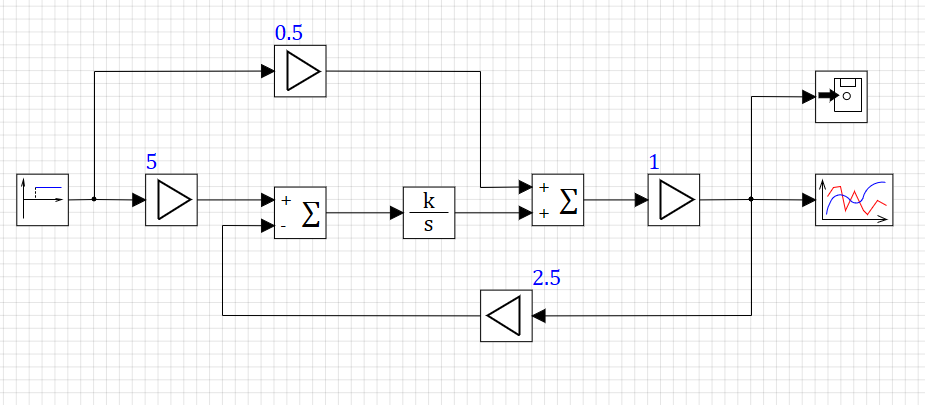
\includegraphics[width=.7\textwidth]{png/scheme1.png}
		\caption{Схема для моделирования упругого звена}
		\label{scheme1}
	\end{figure}
	
	Интегрирование дифференциального уравнения будет проводиться с помощью метода Рунге-Кутты 4-го порядка для различных шагов интегрирования. Сравнение с аналитическим решением полученного переходного процесса приведено на рис. \ref{sravn1}.
	
	\begin{center}
		\noindent\begin{minipage}{.4\textwidth}
			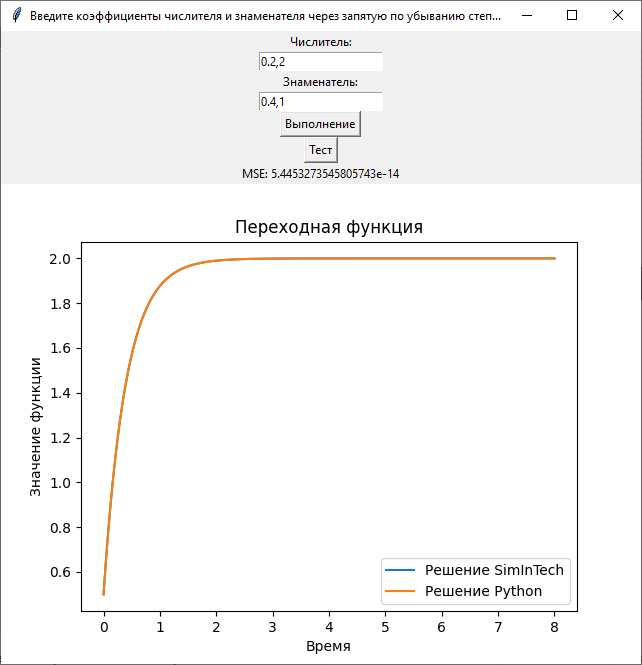
\includegraphics[width=\textwidth]{png/graph1.png}
			\centering{а)}
		\end{minipage}
		\begin{minipage}{.4\textwidth}
			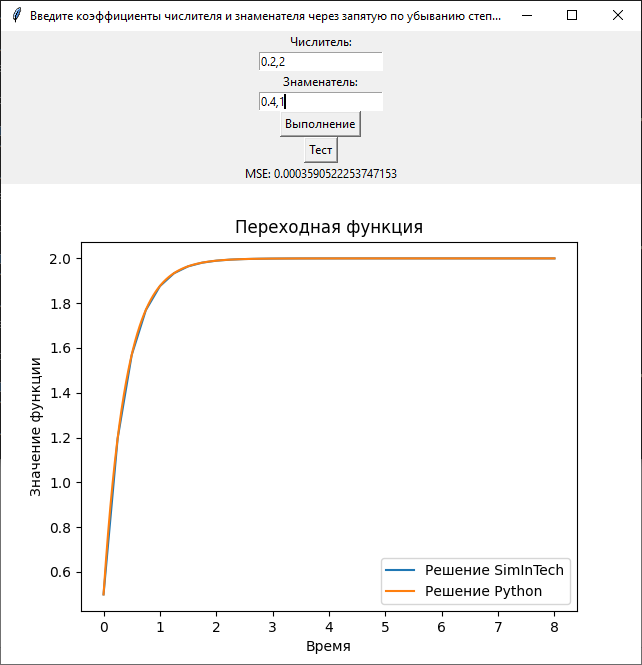
\includegraphics[width=\textwidth]{png/graph2.png}
			\centering{б)}
		\end{minipage}
		\captionof{figure}{Сравнение смоделированного и истинного переходного процесса: а) $\Delta t = 0.001$, б) $\Delta t = 0.25$}
		\label{sravn1}	
	\end{center}
	
	Ошибка моделирования оценивается следующим образом:
	\begin{equation}
		RMSE = \frac{1}{N} \norm{h - \hat{h}}_2 = \frac{1}{N}\sqrt{\sum_{i=1}^N (h_i - \hat{h}_i)^2}
	\end{equation}

	Здесь $h$ - истинные значения переходной функции, $\hat{y}$ - значения, полученные в результате моделирования. График ошибки приведен на рис. \ref{rmse1}.
	
	В результате проведения экспериментов для различных значений шага интегрирования $\Delta t$ были получены следующие значения: табл. \ref{tabl1}.
	
	\begin{filecontents*}{data.csv}
	a,b
	0.001,5.45e-14
	0.01,5.57e-10
	0.1,6.73e-6
	0.2,0.00013
	0.25,0.00036
	\end{filecontents*}

	\begin{center}
		\begin{tikzpicture}
			\begin{axis}[
				xlabel={$\Delta t$},
				ylabel={$RMSE$},
				xtick distance = 0.05,
				xlabel style={above right},
				xmin=0, xmax = 0.28,
				ylabel style = {above right},
				ymin=1e-14, ymax = 80,
				ymode=log,
				axis lines = center,
				clip=false
				]
				\addplot[smooth, tension=0.5, mark=*] table [x=a, y=b, col sep=comma] {data.csv};
				\node [below right] at (0,0) {0};
			\end{axis}
		\end{tikzpicture}
		\captionof{figure}{График зависимости ошибки RMSE моделирования от шага интегрирования}
		\label{rmse1}	
	\end{center}
	
		
	\begin{table}[h]
		\begin{center}
			\begin{tabular}{|c|cc|}
				\hline
				\multirow{2}{*}{Шаг интегрирования $\Delta t$, с} & \multicolumn{2}{c|}{RMSE}                                         \\ \cline{2-3} 
				& \multicolumn{1}{c|}{Упругое звено}        & Колебательное звено  \\ \hline
				0.001                                             & \multicolumn{1}{c|}{$5.45\cdot 10^{-14}$} & $1.01\cdot 10^{-13}$ \\ \hline
				0.01                                              & \multicolumn{1}{c|}{$5.57\cdot 10^{-10}$} & $1.01\cdot 10^{-9}$  \\ \hline
				0.1                                               & \multicolumn{1}{c|}{$6.73\cdot 10^{-6}$}  & $1.06\cdot 10^{-5}$  \\ \hline
				0.2                                               & \multicolumn{1}{c|}{$1.3\cdot 10^{-4}$}   & $1.77\cdot 10^{-4}$  \\ \hline
				0.25                                              & \multicolumn{1}{c|}{$3.6\cdot 10^{-4}$}   & $4.44\cdot 10^{-4}$  \\ \hline
			\end{tabular}
			\caption{Значения ошибки моделирования RMSE от шага интегрирования $\Delta t$}
			\label{table1}
		\end{center}
	\end{table}		
	
	По полученным данным явно видно, что метод Рунге-Кутты 4 порядка в действительности является методом 4-го порядка, так как $10$-кратное увеличение шага интегрирования приводит к $10^4$-кратному увеличению ошибки интегрирования.
	
	\subsection{Колебательное звено}
	
	Звено рассматривается со следующими параметрами:
	\begin{equation*}
		k=5,\;a=1.1,\;b=3.9
	\end{equation*}

	Моделирование будет проводиться в тех же условиях, что и для упругого звена. Схема моделирования приведена на рис. \ref{scheme2}
	
	\begin{figure}[h]
		\centering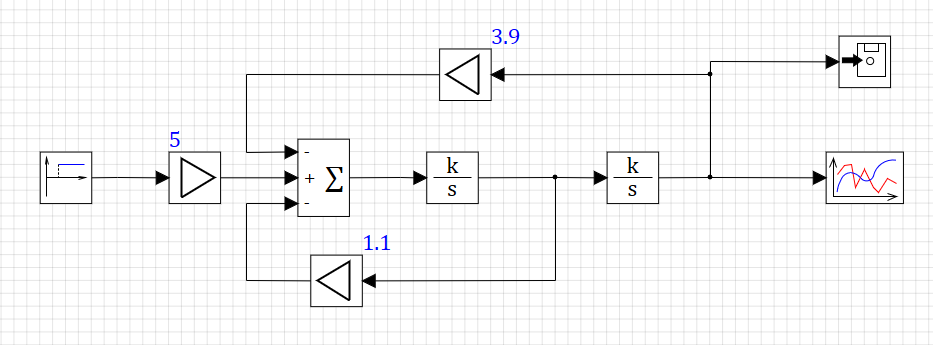
\includegraphics[width=.7\textwidth]{png/scheme2.png}
		\caption{Схема для моделирования колебательного звена}
		\label{scheme2}
	\end{figure}

	Пример переходного процесса для различных шагов интегрирования приведен на рис. \ref{sravn2}
	
	\begin{center}
		\noindent\begin{minipage}{.4\textwidth}
			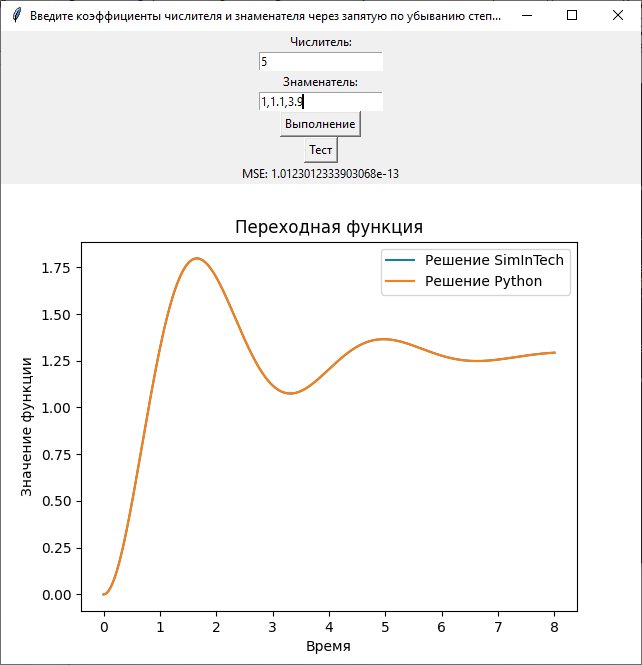
\includegraphics[width=\textwidth]{png/graph3.png}
			\centering{а)}
		\end{minipage}
		\begin{minipage}{.4\textwidth}
			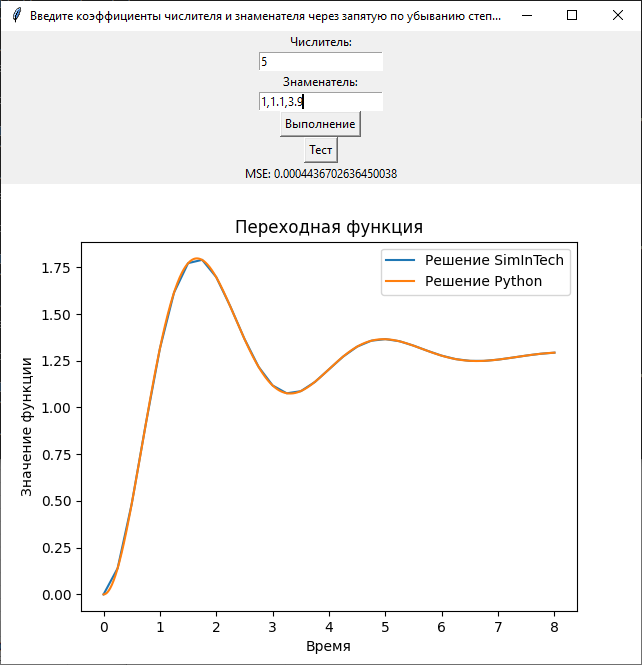
\includegraphics[width=\textwidth]{png/graph4.png}
			\centering{б)}
		\end{minipage}
		\captionof{figure}{Сравнение смоделированного и истинного переходного процесса: а) $\Delta t = 0.001$, б) $\Delta t = 0.25$}
		\label{sravn2}	
	\end{center}
	
	Полученный график ошибки представлен на рис. \ref{rmse2}. Сами значения ошибок приведены в табл. \ref{table1}.
	
	\begin{filecontents*}{data2.csv}
		a,b
		0.001,1.01e-13
		0.01,1.01e-9
		0.1,1.06e-5
		0.2,1.77e-4
		0.25,4.44e-4
	\end{filecontents*}
	
	\begin{center}
		\begin{tikzpicture}
			\begin{axis}[
				xlabel={$\Delta t$},
				ylabel={$RMSE$},
				xtick distance = 0.05,
				xlabel style={above right},
				xmin=0, xmax = 0.28,
				ylabel style = {above right},
				ymin=1e-14, ymax = 80,
				ymode=log,
				axis lines = center,
				clip=false
				]
				\addplot[smooth, tension=0.5, mark=*] table [x=a, y=b, col sep=comma] {data2.csv};
				\node [below right] at (0,0) {0};
			\end{axis}
		\end{tikzpicture}
		\captionof{figure}{График зависимости ошибки RMSE моделирования от шага интегрирования}
		\label{rmse2}	
	\end{center}

	\subsection{Звено с дифференциальным оператором 2-го порядка}
	
	Звено рассматривается со следующими параметрами:
	\begin{equation*}
		a=0.4,\;b=1.1,\;c=2,\;d=6,\;e=2.5
	\end{equation*}
	
	Моделирование проводится в условиях, аналогичных упругому звену. Схема для моделирования приведена на рис. \ref{scheme3}.
	
	\begin{figure}[h]
		\centering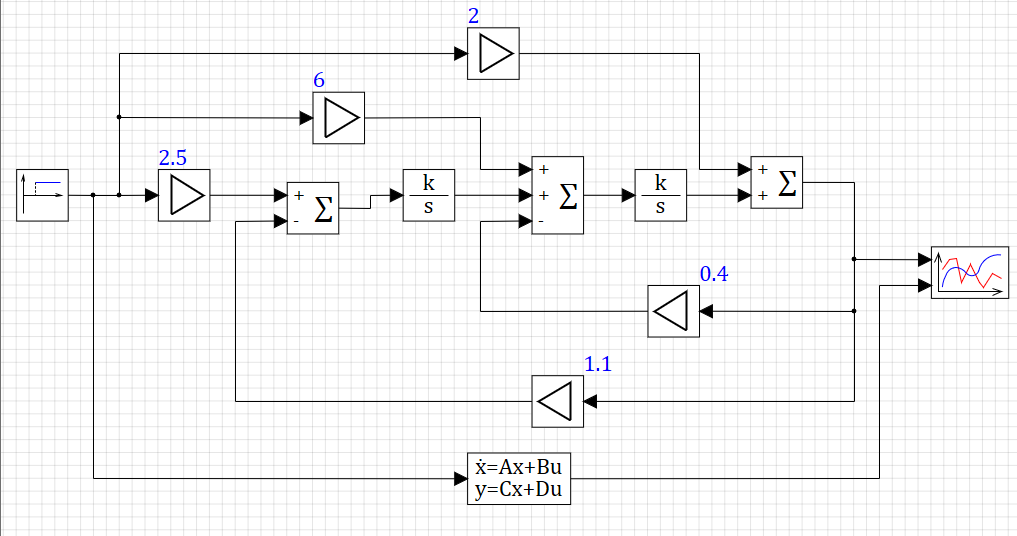
\includegraphics[width=.7\textwidth]{png/scheme3.png}
		\caption{Схема для моделирования звена с дифференциальным оператором 2-го порядка}
		\label{scheme3}
	\end{figure}

	Как видно на рисунке, система была смоделирована как в виде аналоговой структурной схемы, так и в представлении в переменных состояния. Представление в переменных состояния использовалось то же, что было получено в подготовке к работе, с учётом того, что в среде Simintech матрица состояния $A$ вводится в транспонированной форме.
	
	Полученные графики переходного процесса представлены на рис. \ref{graph5}.
	\begin{figure}[h]
		\centering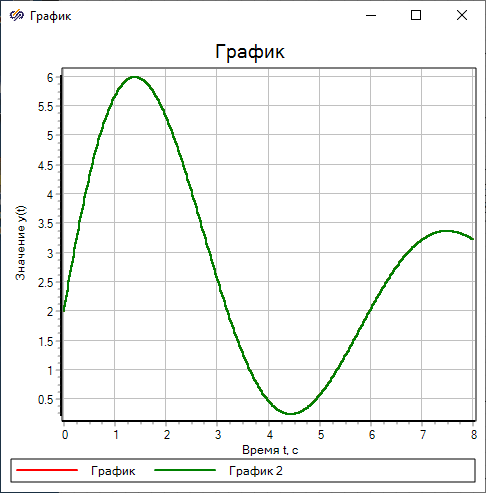
\includegraphics[width=.55\textwidth]{png/graph5.png}
		\caption{Переходной процесс звена с дифференциальным оператором 2-го порядка}
		\label{graph5}
	\end{figure}

	Как видно, процессы полученные в результате моделирования обоими способами совпали.
	
	\section{Выводы}
	
	Было проведено моделирование трёх различных звеньев: упругого, колебательного и звена заданного дифференциальными операторами 2-го порядка. Моделирование проводилось путём представления звеньев в виде аналоговой структурной схемы. Для численного интегрирования использовался метод Рунге-Кутты 4-го порядка, и полученные значения среднеквадратичной ошибки подтвердили, что порядок его точности равен 4.
	
	Также было моделирование последнего звена в представлении в переменных состояния. Полученный переходной процесс совпал с результатом моделирования аналоговой структурной схемы этого звена.
	
\end{document}
